\newpage
\subsection{XYZ-Wing}
Bei der Technik \textit{XYZ-Wing} handelt ies sich um eine erweiterte Version der Technik \textit{XY-Wing}. Zusätzlich zu den Kandidaten x und y steht hier in der ersten Zelle noch der Kandidat z, der Rest ändert sich nicht. Statt zwei Fällen werden hier drei Fälle betrachtet. Wenn der Kandidat x in der ersten Zelle steht, dannn bleibt die Argumentation wie beim \textit{XY-Wing}. Das selbe gilt für den Fall, dass der Kandidat y in der ersten Zelle steht. Im dritten Fall steht der Kandidat z in der ersten Zelle. In diesem Fall würde er alle Kandidaten ausschließen, die von dort aus direkt auschgeschlossen werden. Daher können alle Kandidaten der Ziffer z gelöscht werden, die von allen drei Zellen ausgeschlossen werden.

\begin{figure}[h]
\begin{center}
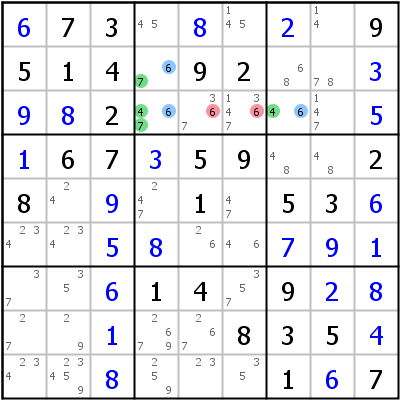
\includegraphics{./img/XYZ_Wing.png}
\caption{XYZ-Wing}
\end{center}
\end{figure}

In \textbf{Abbildung 3.14} sieht man einen \textit{XYZ-Wing}, dessen erste Zelle z3s4 ist. Hier stehen die Kandidaten 4 für x, 7 für y und 6 für z. Bei z3s7 findet man die zweite Zelle mit den Kandidaten 4 und 6, also x und z. Die dritte Zelle ist z2s4, sie enthält die Kandidaten 6 und 7 und damit y und z. Wenn die Ziffer 4 ind z3s4 steht, dann muss in z3s6 die Ziffer 6 stehen und damit sind die rot markierten Kandidaten ausgeschlossen. Wenn in z3s4 die Ziffer 7 steht, dann muss in z2s4 die Ziffer 6 stehen und auch in diesem Fall sind die rot markierten Kandidaten ausgeschlossen. Wenn in z3s4 die Ziffer 6 steht, dann sind ebenfalls die rot markierten Kandidaten ausgschlossen. Somit können sie in jedem der möglichen Fälle ausgeschlossen werden und werden daher gelöscht.